
\documentclass[12pt,a4paper]{article}
\usepackage{basilisk_i18n}
\usepackage{needspace}

\BusinessPlanCompany{Spectrum AI}
\BusinessPlanWatermarkText{Spectrum AI}
\BusinessPlanWatermarkColor{black!6}
\BusinessPlanWatermarkFontSize{38}{46}
\BusinessPlanWatermarkAngle{38}
\BusinessPlanAuthorsText{Spectrum AI --- dokument roboczy dla założycieli}
\BusinessPlanConfidentialText{Dokument roboczy --- komentarze nie stanowią tekstu umowy}
\BusinessPlanFooterText{Spectrum AI --- umowa sp. z o.o. / wersja robocza}
\BusinessPlanVersionText{Wersja robocza}

\setstretch{1.18}
\setlist[itemize]{topsep=0.2em,itemsep=0.15em,parsep=0.1em}
\setlist[enumerate]{topsep=0.25em,itemsep=0.18em,parsep=0.1em}

\newcounter{paragraf}
\newcommand{\paragraf}[1]{%
  \refstepcounter{paragraf}%
  \phantomsection%
  \addcontentsline{toc}{section}{\S~\theparagraf\ #1}%
  \Needspace{6\baselineskip}%
  \subsection*{\S~\theparagraf\ #1}%
}

\tcbset{
  basiliskbox/.style={enhanced, breakable, sharp corners=south, arc=1mm, boxrule=0.5pt, left=7pt, right=7pt, top=7pt, bottom=7pt, before skip=8pt, after skip=10pt},
}

\newenvironment{ContractClause}[1]{%
  \begin{tcolorbox}[basiliskbox, colback=white, colframe=black!70, coltitle=white, fonttitle=\bfseries, title={TEKST UMOWY --- #1}]%
  \paragraf{#1}%
}{%
  \end{tcolorbox}%
}

\newcommand{\DiscussionComment}[2]{%
  \begin{tcolorbox}[basiliskbox, colback=orange!6, colframe=orange!70!black, coltitle=black, fonttitle=\bfseries, title={KOMENTARZ DO DYSKUSJI --- #1}]%
  \textbf{Status: materiał do rozmowy na posiedzeniu założycielskim. Nie jest częścią tekstu umowy.}\par\smallskip
  #2%
  \end{tcolorbox}%
}

\newenvironment{DiscussionGraphic}[1]{%
  \begin{tcolorbox}[basiliskbox, colback=blue!4, colframe=blue!55!black, coltitle=black, fonttitle=\bfseries, title={GRAFIKA DO DYSKUSJI --- #1}]%
  \textbf{Status: ilustracja robocza. Nie jest częścią tekstu umowy.}\par\smallskip
}{%
  \end{tcolorbox}%
}

\newcommand{\MeetingDecision}[1]{\textbf{Decyzja do podjęcia:} #1}

\begin{document}

\BusinessPlanTitlePage
  {Spectrum AI}
  {Pakiet na posiedzenie założycielskie}
  {Umowa spółki z o.o. z komentarzami}
  {Projekt umowy Spółki z ograniczoną odpowiedzialnością}
  {Wyraźnie oddzielono tekst umowy od komentarzy i grafik do dyskusji}
  {0.2}

\tableofcontents
\newpage

\section*{Instrukcja użycia na posiedzeniu założycielskim}
\addcontentsline{toc}{section}{Instrukcja użycia na posiedzeniu założycielskim}

\begin{tcolorbox}[basiliskbox, colback=green!5, colframe=green!45!black, title={LEGENDA DOKUMENTU}, fonttitle=\bfseries]
\begin{itemize}[leftmargin=*]
  \item Ramki \textbf{TEKST UMOWY} zawierają projekt paragrafów, które mogą wejść do umowy spółki.
  \item Ramki \textbf{KOMENTARZ DO DYSKUSJI} są roboczym materiałem dla założycieli i nie powinny być podpisywane jako treść umowy.
  \item Ramki \textbf{GRAFIKA DO DYSKUSJI} są ilustracjami decyzyjnymi: cap table, organy, vesting, transakcje udziałowe i deadlock.
  \item Przed podpisaniem należy usunąć komentarze oraz grafiki albo przenieść je do protokołu posiedzenia / listy ustaleń.
\end{itemize}
\end{tcolorbox}


\begin{DiscussionGraphic}{jak czytać dokument}
\centering
\begin{tikzpicture}[>=Latex, node distance=1.4cm, box/.style={draw, rounded corners, align=center, minimum width=4.8cm, minimum height=1.0cm}]
  \node[box, fill=black!5] (contract) {TEKST UMOWY\\paragrafy do podpisania};
  \node[box, fill=orange!10, right=of contract] (comment) {KOMENTARZE\\materiał do dyskusji};
  \node[box, fill=blue!7, below=of contract] (graphic) {GRAFIKI\\ułatwiają decyzje};
  \node[box, fill=green!7, below=of comment] (meeting) {POSIEDZENIE\\ustalenia i poprawki};
  \draw[->] (contract) -- (meeting);
  \draw[->] (comment) -- (meeting);
  \draw[->] (graphic) -- (meeting);
\end{tikzpicture}
\end{DiscussionGraphic}


\section*{Agenda posiedzenia założycielskiego}
\addcontentsline{toc}{section}{Agenda posiedzenia założycielskiego}
\begin{tcolorbox}[basiliskbox, colback=yellow!5, colframe=yellow!55!black, title={PROPONOWANY PORZĄDEK OBRAD}, fonttitle=\bfseries]
\begin{enumerate}[leftmargin=*]
  \item Potwierdzenie nazwy, siedziby, PKD i zakresu działalności.
  \item Potwierdzenie wspólników, udziałów, wkładów i zasad finansowania.
  \item Ustalenie Zarządu, reprezentacji, spraw zastrzeżonych i deadlocku.
  \item Omówienie IP, poufności, infrastruktury technicznej i zakazu konkurencji.
  \item Omówienie vestingu, lock-upu, tag-along, drag-along i zasad wyceny.
  \item Zatwierdzenie listy poprawek do wersji podpisywanej.
\end{enumerate}
\end{tcolorbox}

\newpage
\section*{Projekt tekstu umowy z komentarzami}
\addcontentsline{toc}{section}{Projekt tekstu umowy z komentarzami}

\begin{ContractClause}{Nazwa Spółki}
\begin{enumerate}
  \item \textbf{Nazwa Spółki brzmi:} Spectrum AI -- sztuczna inteligencja, oprogramowanie, spółka z ograniczoną odpowiedzialnością.
  \item Spółka może używać w obrocie skrótu: \textbf{Spectrum AI sp. z o.o.}
\end{enumerate}
\end{ContractClause}
\DiscussionComment{nazwa i identyfikacja spółki}{
\begin{itemize}[leftmargin=*]
  \item Tekst umowy: zostawić tylko finalną, notarialnie akceptowaną nazwę. Wariant skrócony powinien być spójny z brandingiem i przyszłymi domenami.
  \item Do decyzji: czy nazwa ma pozostać ``Spectrum AI, czy dokument jest jedynie roboczo przenoszony do szablonu Basilisk.
\end{itemize}
}

\begin{ContractClause}{Siedziba Spółki}
\begin{enumerate}
  \item \textbf{Siedzibą Spółki jest} \textbf{Pruszków}, województwo Mazowieckie.
  \item Spółka działa na terytorium Rzeczypospolitej Polskiej i za granicą.
\end{enumerate}
\end{ContractClause}
\DiscussionComment{siedziba i zakres działania}{
\begin{itemize}[leftmargin=*]
  \item Do potwierdzenia na posiedzeniu: miejscowość siedziby, adres do KRS, adres korespondencyjny oraz osoba odpowiedzialna za odbiór korespondencji.
  \item Komentarz nie jest częścią umowy: można dodać osobną uchwałę o dokładnym adresie, aby sama umowa wskazywała tylko miejscowość.
\end{itemize}
}

\begin{ContractClause}{Przedmiot działalności Spółki}
\textbf{Przedmiotem działalności Spółki jest prowadzenie działalności w zakresie:}
\begin{enumerate}
  \item Tworzenia, rozwoju i wdrażania systemów sztucznej inteligencji i uczenia maszynowego \textbf{(PKD 62.01.Z)}.
  \item Projektowania, tworzenia i sprzedaży oprogramowania aplikacyjnego i systemowego \textbf{(PKD 62.01.Z)}.
  \item Działalności portali internetowych i platform cyfrowych \textbf{(PKD 63.12.Z)}.
  \item Sprzedaży detalicznej prowadzonej przez Internet \textbf{(PKD 47.91.Z)}.
  \item Usług chmurowych, hostingu i przetwarzania danych \textbf{(PKD 63.11.Z)}.
  \item Konsultingu technologicznego i integracji systemów \textbf{(PKD 62.02.Z)}.
  \item Działalności badawczo-rozwojowej w zakresie AI i technologii informatycznych \textbf{(PKD 72.19.Z)}.
  \item Produkcji urządzeń elektronicznych i komponentów komputerowych \textbf{(PKD 26.11.Z, 26.20.Z)}.
  \item Działalności wydawniczej i szkoleniowej w zakresie oprogramowania i technologii \textbf{(PKD 58.29.Z, 85.59.B)}.
  \item Nabywania i posiadania udziałów oraz akcji w innych spółkach, w tym PSA \textbf{(PKD 64.20.Z)}.
\end{enumerate}
\end{ContractClause}
\DiscussionComment{PKD i zakres działalności}{
\begin{itemize}[leftmargin=*]
  \item Sprawdzić, czy lista PKD jest wystarczająca dla AI, SaaS, hostingu, e-commerce, R\&D, sprzętu oraz udziałów w innych spółkach.
  \item Do dyskusji: wybrać przedmiot przeważającej działalności i ograniczyć listę tylko do pozycji, które rzeczywiście będą potrzebne przy starcie.
\end{itemize}
}

\begin{ContractClause}{Kapitał zakładowy}
\begin{enumerate}
  \item \textbf{Kapitał zakładowy Spółki wynosi 5\,000 zł} i dzieli się na 100 udziałów o wartości nominalnej 50 zł każdy.
  \item Podwyższenie kapitału zakładowego do kwoty 500\,000 zł w terminie do 2030 roku nie stanowi zmiany umowy Spółki.
\end{enumerate}
\end{ContractClause}
\DiscussionComment{kapitał i przyszłe podwyższenie}{
\begin{itemize}[leftmargin=*]
  \item Do dyskusji: czy 5~000 zł wystarczy operacyjnie, czy wspólnicy wolą rozdzielić finansowanie przez pożyczki, dopłaty lub przyszłą rundę.
  \item Klauzula podwyższenia do 500~000 zł bez zmiany umowy powinna zostać sprawdzona przez prawnika/notariusza przed podpisaniem.
\end{itemize}
}

\begin{ContractClause}{Udziały w Spółce}
\begin{enumerate}
  \item \textbf{Udziały w Spółce są równe i niepodzielne.} Każdy wspólnik może posiadać więcej niż jeden udział.
  \item Na każdy udział przypada jeden głos.
\end{enumerate}
\end{ContractClause}

\begin{ContractClause}{Podział początkowy udziałów}
\begin{enumerate}
  \item \textbf{Wspólnik A} obejmuje 50 udziałów o łącznej wartości nominalnej 2\,500 zł.
  \item \textbf{Wspólnik B} obejmuje 20 udziałów o łącznej wartości nominalnej 1\,000 zł.
  \item \textbf{Wspólnik C} obejmuje 10 udziałów o łącznej wartości nominalnej 500 zł.
  \item \textbf{Wspólnik D} obejmuje 10 udziałów o łącznej wartości nominalnej 500 zł.
  \item \textbf{Wspólnik E} obejmuje 10 udziałów o łącznej wartości nominalnej 500 zł.
\end{enumerate}
\end{ContractClause}
\DiscussionComment{cap table założycielski}{
\begin{itemize}[leftmargin=*]
  \item Uzupełnić prawdziwe dane wspólników zamiast oznaczeń A--E.
  \item Do decyzji: czy podział 50/20/10/10/10 jest docelowy, czy ma być połączony z vestingiem, lock-upem albo dodatkowymi umowami wspólników.
\end{itemize}
}

\begin{DiscussionGraphic}{proponowany podział udziałów}
\centering
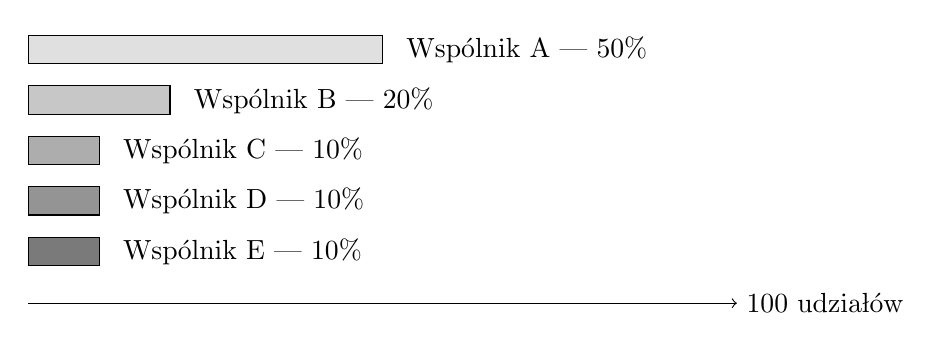
\begin{tikzpicture}[x=0.09cm,y=0.8cm]
  \draw[fill=black!12] (0,0) rectangle (50,0.45);  \node[anchor=west] at (52,0.22) {Wspólnik A --- 50\%};
  \draw[fill=black!22] (0,-0.8) rectangle (20,-0.35); \node[anchor=west] at (22,-0.58) {Wspólnik B --- 20\%};
  \draw[fill=black!32] (0,-1.6) rectangle (10,-1.15); \node[anchor=west] at (12,-1.38) {Wspólnik C --- 10\%};
  \draw[fill=black!42] (0,-2.4) rectangle (10,-1.95); \node[anchor=west] at (12,-2.18) {Wspólnik D --- 10\%};
  \draw[fill=black!52] (0,-3.2) rectangle (10,-2.75); \node[anchor=west] at (12,-2.98) {Wspólnik E --- 10\%};
  \draw[->] (0,-3.8) -- (100,-3.8) node[right]{100 udziałów};
\end{tikzpicture}
\end{DiscussionGraphic}

\begin{ContractClause}{Pokrycie udziałów}
\begin{enumerate}
  \item Udziały w Spółce są pokrywane wkładami pieniężnymi.
  \item \label{pokrycie_sprzętem} Dopuszcza się pokrycie udziałów wkładami niepieniężnymi (aportami),
        jednak wyłącznie w postaci sprzętu lub wyposażenia, którego wartość
        może zostać w sposób jednoznaczny i obiektywny ustalona na podstawie
        cen rynkowych lub dokumentów zakupu.
  \item Wartość wkładu niepieniężnego w postaci sprzętu ustala wspólnik
        wnoszący aport na podstawie dokumentów zakupu lub cen rynkowych,
        a zarząd potwierdza jej prawidłowość w oświadczeniu o wniesieniu wkładów.
  \item \textbf{Wkłady niepieniężne inne niż wskazane w ust. \ref{pokrycie_sprzętem} nie są dopuszczalne (np. prawa autorskie, patenty, prawa majątkowe, know-how)}.
  \item Wspólnicy oświadczają, że sprzęt lub wyposażenie przekazywane Spółce 
      nie jest obciążone prawami osób trzecich, nie stanowi przedmiotu 
      zabezpieczeń ani toczących się postępowań, które mogłyby ograniczyć 
      przeniesienie jego własności na Spółkę. W przypadku zgłoszenia roszczeń 
      przez osoby trzecie, wspólnik przekazujący sprzęt zobowiązuje się do 
      naprawienia szkody poniesionej przez Spółkę.

\end{enumerate}
\end{ContractClause}
\DiscussionComment{wkłady pieniężne, aport sprzętu i IP}{
\begin{itemize}[leftmargin=*]
  \item Tekst wyłącza prawa autorskie, patenty, know-how i inne IP jako aport. To jest dobre organizacyjnie, ale wymaga osobnych umów przeniesienia praw.
  \item Do przygotowania przed podpisaniem: tabela wkładów pieniężnych, ewentualny wykaz sprzętu, dowody zakupu i potwierdzenie braku obciążeń.
\end{itemize}
}

\begin{ContractClause}{Zbycie i zastawienie udziałów}
\begin{enumerate}
  \item Zbycie oraz zastawienie udziału wymaga zgody Spółki udzielanej przez Zarząd na piśmie.
  \item Zastawnik i użytkownik mogą wykonywać prawo głosu z udziału, jeżeli przewiduje to czynność prawna oraz dokonano odpowiedniej wzmianki w księdze udziałów.
\end{enumerate}
\end{ContractClause}

\begin{ContractClause}{Kapitały rezerwowy i zapasowy}
\begin{enumerate}
  \item Spółka może tworzyć kapitały rezerwowy i zapasowy.
  \item Zarząd może wypłacić zaliczkę na poczet przewidywanej dywidendy, jeżeli spełnione są warunki ustawowe.
\end{enumerate}
\end{ContractClause}

\begin{ContractClause}{Rezerwy obligatoryjne}
\begin{enumerate}
  \item Spółka tworzy obowiązkowo kapitał rezerwowy w wysokości co najmniej 10\% rocznego zysku netto.
  \item Kapitał rezerwowy przeznacza się na inwestycje w spółki zależne oraz rozwój działalności Spółki.
  \item Wspólnicy mogą podjąć uchwałę o zwiększeniu wysokości obowiązkowej rezerwy.
\end{enumerate}
\end{ContractClause}

\begin{ContractClause}{Dziedziczenie udziałów}
\begin{enumerate}
  \item \label{zgoda_na_nabycie:ust1} Nabycie udziałów w drodze dziedziczenia wymaga zgody Spółki udzielanej przez Zarząd na piśmie, chyba że zgody tej udzieli Zgromadzenie Wspólników. Zarząd udziela zgody albo odmawia jej udzielenia w terminie 30 dni od dnia otrzymania zawiadomienia o nabyciu spadku w drodze dziedziczenia.

  \item Do czasu zakończenia postępowania spadkowego spadkobiercy mogą wykonywać jedynie prawa majątkowe z udziałów, natomiast prawa korporacyjne, w tym prawo głosu, są zawieszone.

  \item W przypadku odmowy udzielenia zgody, o której mowa w ust. \ref{zgoda_na_nabycie:ust1}, Spółka jest zobowiązana wskazać nabywcę udziałów oraz zapewnić spadkobiercom zapłatę wartości udziałów odpowiadającej ich wartości godziwej. Zarząd dokonuje wskazania nabywcy oraz zapewnia zapłatę w terminie 30 dni od dnia odmowy udzielenia zgody.

  \item Do czasu przeniesienia udziałów na wskazanego nabywcę spadkobiercy zachowują prawa majątkowe z udziałów, jednak nie wykonują praw korporacyjnych.
\end{enumerate}
\end{ContractClause}

\begin{ContractClause}{Ochrona płynności Spółki w przypadku śmierci lub rozwodu wspólnika}
\begin{enumerate}
  \item W przypadku śmierci wspólnika lub podziału majątku wspólnego małżonków
        obejmującego udziały w Spółce, Spółka nie jest zobowiązana do natychmiastowej
        wypłaty wartości udziałów, jeżeli mogłoby to zagrozić jej płynności finansowej
        lub zdolności do kontynuowania działalności.

  \item \label{wyplata_za_udzialy} Wypłata wartości udziałów spadkobiercom lub byłemu małżonkowi może zostać
        rozłożona na raty na okres nie dłuższy niż 36 miesięcy, chyba że strony
        uzgodnią inaczej. Terminy i wysokość rat ustala Zarząd, kierując się
        sytuacją finansową Spółki.

  \item Do czasu całkowitej spłaty udziałów spadkobiercy lub były małżonek nie
        wykonują praw korporacyjnych, a jedynie prawa majątkowe, o ile umowa
        Spółki nie stanowi inaczej.

  \item \label{nie_moge_splacic} Jeżeli sytuacja finansowa Spółki nie pozwala na dokonanie wypłaty wartości
        udziałów w terminach określonych w ust. \ref{wyplata_za_udzialy}, spadkobierca lub były małżonek
        automatycznie staje się wspólnikiem Spółki z chwilą upływu terminu płatności
        pierwszej raty, której Spółka nie jest w stanie uiścić, bez konieczności
        podejmowania dodatkowej uchwały.
        
 \item W przypadku, o którym mowa w ust. \ref{nie_moge_splacic}, liczba udziałów obejmowanych
        przez spadkobiercę lub byłego małżonka zostaje pomniejszona proporcjonalnie
        o udziały, za które Spółka dokonała już częściowej spłaty.        

  \item Spółka może zawrzeć ze spadkobiercami lub byłym małżonkiem porozumienie
        przewidujące odroczenie, rozłożenie na raty lub obniżenie wynagrodzenia
        za udziały, jeżeli jest to konieczne dla zachowania płynności Spółki.
\end{enumerate}
\end{ContractClause}

\begin{ContractClause}{Organy Spółki}
\begin{enumerate}
  \item Organami Spółki są:
    \begin{enumerate}
      \item Zarząd -- organ prowadzący sprawy Spółki i reprezentujący ją na zewnątrz,
      \item Rada Nadzorcza -- organ sprawujący stały nadzór nad działalnością Spółki (jeżeli została ustanowiona),
      \item Zgromadzenie Wspólników -- najwyższy organ Spółki, uprawniony do podejmowania uchwał w sprawach określonych przepisami prawa oraz niniejszą umową.
    \end{enumerate}
\end{enumerate}
\end{ContractClause}
\DiscussionComment{model organów}{
\begin{itemize}[leftmargin=*]
  \item Ustalić, czy Rada Nadzorcza ma być realnie powołana od początku, czy tylko opisana jako organ opcjonalny.
  \item Do decyzji: kto będzie pierwszym Zarządem i czy Prezes ma mieć decydujący głos przy sporach.
\end{itemize}
}

\begin{DiscussionGraphic}{schemat organów i odpowiedzialności}
\centering
\begin{tikzpicture}[node distance=1.35cm, >=Latex, box/.style={draw, rounded corners, align=center, minimum width=4.4cm, minimum height=0.9cm, fill=black!5}]
  \node[box] (w) {Zgromadzenie\\Wspólników};
  \node[box, below=of w] (z) {Zarząd\\prowadzenie spraw i reprezentacja};
  \node[box, below left=1.0cm and 1.4cm of z] (rn) {Rada Nadzorcza\\opcjonalnie};
  \node[box, below right=1.0cm and 1.4cm of z] (sp) {Spółka\\operacje, IP, finanse};
  \draw[->] (w) -- node[right]{powołuje / uchwały} (z);
  \draw[->] (rn) -- node[below]{nadzór} (sp);
  \draw[->] (z) -- node[right]{zarządza} (sp);
\end{tikzpicture}
\end{DiscussionGraphic}

\begin{ContractClause}{Zarząd Spółki}
\begin{enumerate}
  \item Zarząd składa się z jednego lub więcej członków powoływanych uchwałą wspólników.
  \item Kadencja członka Zarządu wynosi 5 lat.
  \item Mandat wygasa z chwilą upływu kadencji, odwołania, śmierci albo rezygnacji.
  \item Jeżeli Zarząd jest wieloosobowy, Zgromadzenie Wspólników może powołać spośród członków Zarządu Prezesa Zarządu.
  \item Prezes Zarządu koordynuje pracę Zarządu, zwołuje posiedzenia Zarządu oraz przewodniczy ich obradom.
  \item W przypadku równej liczby głosów przy podejmowaniu uchwał Zarządu decyduje głos Prezesa Zarządu, o ile został powołany.
  \item Prezes Zarządu może wydawać wytyczne organizacyjne dotyczące bieżącego funkcjonowania Spółki, o ile nie naruszają one kompetencji pozostałych organów Spółki ani uchwał Zgromadzenia Wspólników.
\end{enumerate}
\end{ContractClause}

\begin{ContractClause}{Uprawnienia Zarządu}
\begin{enumerate}
  \item Zarząd prowadzi sprawy Spółki i reprezentuje ją na zewnątrz we wszystkich czynnościach sądowych i pozasądowych.
  \item Do kompetencji Zarządu należy w szczególności:
    \begin{enumerate}
      \item podejmowanie decyzji dotyczących bieżącej działalności Spółki,
      \item sporządzanie rocznych sprawozdań finansowych oraz sprawozdań z działalności Spółki,
      \item przygotowywanie projektów uchwał dla Zgromadzenia Wspólników,
      \item nabywanie, zbywanie i obciążanie składników majątku Spółki, z zastrzeżeniem spraw zastrzeżonych do kompetencji Zgromadzenia Wspólników,
      \item ustanawianie prokury oraz pełnomocników Spółki,
      \item zawieranie umów o pracę oraz innych umów cywilnoprawnych z pracownikami i współpracownikami Spółki,
      \item podejmowanie decyzji inwestycyjnych w granicach zwykłego zarządu.
    \end{enumerate}
  \item Uchwały Zarządu zapadają zwykłą większością głosów, chyba że umowa Spółki stanowi inaczej.
  \item W przypadku równej liczby głosów decyduje głos Prezesa Zarządu, jeżeli został powołany.
\end{enumerate}
\end{ContractClause}

\begin{ContractClause}{Sprawy Organizacyjne}
\begin{enumerate}
  \item Zarząd może uchwalić regulamin określający szczegółowy tryb pracy Zarządu, podział obowiązków między członków Zarządu oraz zasady podejmowania decyzji.
  \item Spółka prowadzi księgi rachunkowe zgodnie z obowiązującymi przepisami prawa.
  \item Rok obrotowy Spółki pokrywa się z rokiem kalendarzowym, chyba że Zgromadzenie Wspólników postanowi inaczej.
  \item Dokumenty Spółki mogą być prowadzone i przechowywane w formie papierowej lub elektronicznej.
  \item Spółka może tworzyć oddziały, przedstawicielstwa oraz inne jednostki organizacyjne na terytorium Rzeczypospolitej Polskiej i poza jej granicami.
  \item Wszelkie zmiany adresu siedziby Spółki w obrębie tej samej miejscowości nie stanowią zmiany umowy Spółki.
\end{enumerate}
\end{ContractClause}

\begin{ContractClause}{Reprezentacja Spółki}
\begin{enumerate}
  \item W przypadku Zarządu jednoosobowego oświadczenia w imieniu Spółki składa członek Zarządu.
  \item W przypadku Zarządu wieloosobowego wymagane jest współdziałanie dwóch członków Zarządu albo jednego członka Zarządu łącznie z prokurentem.
\item Członek Zarządu nie może reprezentować Spółki przy dokonywaniu czynności prawnych z samym sobą ani jako pełnomocnik innej osoby, chyba że czynność ta polega na spełnieniu świadczenia wynikającego z istniejącego stosunku prawnego. W takich przypadkach Spółkę reprezentuje inny członek Zarządu. Członek Zarządu jest ponadto zobowiązany powstrzymać się od reprezentowania Spółki w sprawach, w których zachodzi konflikt interesów między nim a Spółką, a w takim przypadku Spółkę reprezentuje inny członek Zarządu.
\end{enumerate}
\end{ContractClause}
\DiscussionComment{reprezentacja i konflikt interesów}{
\begin{itemize}[leftmargin=*]
  \item Do potwierdzenia: reprezentacja jednoosobowa przy jednoosobowym Zarządzie oraz łączna przy Zarządzie wieloosobowym.
  \item Warto dopisać praktyczną procedurę dla umów z członkiem Zarządu: pełnomocnik wspólników, uchwała, protokół, archiwizacja.
\end{itemize}
}

\begin{ContractClause}{Zasady wypłaty dywidendy}
\begin{enumerate}
  \item Dywidenda może być wypłacona wspólnikom wyłącznie na podstawie uchwały Zgromadzenia Wspólników, podjętej po zatwierdzeniu sprawozdania finansowego za dany rok obrotowy oraz po stwierdzeniu istnienia zysku przeznaczonego do podziału.

  \item Jeżeli uchwała Zgromadzenia Wspólników nie stanowi inaczej, dniem wypłaty dywidendy jest rocznica wpisu Spółki do rejestru przedsiębiorców Krajowego Rejestru Sądowego („urodziny Spółki”).

  \item Zgromadzenie Wspólników może w uchwale określić inny dzień dywidendy lub inny termin wypłaty dywidendy.

  \item Dywidenda jest wypłacana wspólnikom proporcjonalnie do posiadanych udziałów, chyba że uchwała Zgromadzenia Wspólników stanowi inaczej w granicach dopuszczonych przez przepisy prawa.

  \item Wypłata dywidendy nie może naruszać wypłacalności Spółki ani zagrażać jej dalszemu funkcjonowaniu. Zarząd jest zobowiązany do dokonania oceny wypłacalności Spółki przed dokonaniem wypłaty dywidendy.

  \item Jeżeli po podjęciu uchwały o wypłacie dywidendy, a przed jej wypłatą, wystąpią okoliczności wskazujące na zagrożenie wypłacalności Spółki, Zarząd może wstrzymać wypłatę dywidendy do czasu ustania zagrożenia, informując o tym niezwłocznie wspólników wraz z uzasadnieniem.

  \item Spółka może wypłacać wspólnikom zaliczkę na poczet przewidywanej dywidendy, jeżeli spełnione są warunki określone w Kodeksie spółek handlowych, a Zarząd stwierdzi, że sytuacja finansowa Spółki na to pozwala.

  \item Wspólnicy mogą postanowić o przeznaczeniu całości lub części zysku na:
    \begin{enumerate}
      \item kapitał zapasowy lub rezerwowy,
      \item inwestycje Spółki,
      \item pokrycie strat z lat ubiegłych,
      \item inne cele określone uchwałą Zgromadzenia Wspólników.
    \end{enumerate}

  \item Dywidenda wypłacana jest na rachunek bankowy wskazany przez wspólnika, chyba że Zgromadzenie Wspólników postanowi inaczej.
\end{enumerate}
\end{ContractClause}
\DiscussionComment{dywidenda i reinwestowanie zysku}{
\begin{itemize}[leftmargin=*]
  \item Do decyzji: czy ``urodziny Spółki jako domyślny dzień wypłaty dywidendy zostają, czy lepiej pozostawić termin wyłącznie uchwale wspólników.
  \item Ustalić politykę: najpierw rezerwa / reinwestycje / spłata pożyczek, a dopiero potem dywidenda.
\end{itemize}
}

\begin{ContractClause}{Wyjście ze Spółki}
\begin{enumerate}
  \item Wspólnik może żądać odkupu jego udziałów przez Spółkę lub pozostałych wspólników w przypadku:
    \begin{enumerate}
      \item braku wypłaty dywidendy przez okres 3 kolejnych lat,
      \item zmiany przedmiotu działalności Spółki w sposób istotny,
      \item podjęcia uchwały o sprzedaży większości udziałów w spółkach zależnych.
    \end{enumerate}
  \item Cena odkupu udziałów ustalana jest na podstawie wyceny niezależnego biegłego rewidenta.
\end{enumerate}
\end{ContractClause}

\begin{ContractClause}{Prawo pierwszeństwa}
\begin{enumerate}
  \item W przypadku zamiaru zbycia udziałów przez wspólnika, pozostali wspólnicy mają prawo pierwszeństwa ich nabycia na warunkach równych z oferowanymi osobom trzecim.
  \item Prawo pierwszeństwa wykonywane jest w terminie 30 dni od dnia zawiadomienia wspólników o zamiarze zbycia udziałów.
  \item W przypadku niewykonania prawa pierwszeństwa w terminie, wspólnik może zbyć udziały osobie trzeciej na warunkach niekorzystniejszych niż zaoferowane wspólnikom.
\end{enumerate}
\end{ContractClause}

\begin{ContractClause}{Likwidacja Spółki}
\begin{enumerate}
  \item Likwidacja Spółki następuje na podstawie uchwały wspólników lub z innych przyczyn przewidzianych prawem.
  \item Majątek pozostały po zaspokojeniu wierzycieli dzieli się pomiędzy wspólników proporcjonalnie do posiadanych udziałów.
\end{enumerate}
\end{ContractClause}

\begin{ContractClause}{Własność intelektualna}
\begin{enumerate}
  \item Wspólnicy oświadczają, że wszelkie prawa własności intelektualnej 
        (w tym autorskie prawa majątkowe, prawa do wynalazków, wzorów użytkowych, 
        wzorów przemysłowych, znaków towarowych, know-how oraz prawa do baz danych) 
        powstałe przed dniem zawarcia niniejszej umowy, a także powstałe w trakcie 
        trwania stosunku ze Spółką, które dotyczą przedmiotu działalności Spółki, 
        zostają przeniesione na Spółkę na podstawie odrębnych umów, o których mowa 
        w ust. \ref{prawa_autorskie}. Prawa te nie stanowią wkładu na kapitał zakładowy Spółki.

  \item \label{prawa_autorskie} Wspólnicy zobowiązują się do niezwłocznego zawarcia odrębnych umów 
        przenoszących prawa autorskie, prawa pokrewne oraz inne prawa własności 
        intelektualnej na rzecz Spółki, w tym do złożenia oświadczeń i podpisania 
        dokumentów niezbędnych do dokonania wpisów w odpowiednich rejestrach 
        i urzędach.

  \item Wspólnicy oświadczają, że prawa własności intelektualnej przenoszone na 
        Spółkę nie są obciążone prawami osób trzecich, nie stanowią przedmiotu 
        zabezpieczeń ani toczących się postępowań, które mogłyby ograniczyć ich 
        przeniesienie. W przypadku zgłoszenia roszczeń przez osoby trzecie, 
        wspólnik przenoszący prawa zobowiązuje się do naprawienia szkody 
        poniesionej przez Spółkę.

  \item Prawa własności intelektualnej, know-how, oprogramowanie, dane, modele AI, 
        dokumentacja techniczna oraz inne wartości niematerialne i prawne nie mogą 
        być wnoszone do Spółki jako wkład na kapitał zakładowy ani jako wkład 
        niepieniężny.

\end{enumerate}
\end{ContractClause}
\DiscussionComment{IP jako osobny pakiet dokumentów}{
\begin{itemize}[leftmargin=*]
  \item Komentarz nie jest częścią umowy: przygotować osobne umowy przeniesienia praw autorskich, know-how, kodu, modeli AI, baz danych i dokumentacji.
  \item Do dyskusji: czy prawa stworzone przed zawarciem umowy mają być przenoszone w całości, licencjonowane, czy wyłączone z majątku spółki.
\end{itemize}
}

\begin{ContractClause}{Nabywanie praw do udziałów (vesting)}
\begin{enumerate}
  \item Udziały przydzielone Wspólnikowi podlegają mechanizmowi nabywania praw (vesting), co oznacza, że Wspólnik uzyskuje prawa korporacyjne i majątkowe do udziałów stopniowo, zgodnie z niniejszym paragrafem.

  \item Okres nabywania praw oznacza czas, w którym Wspólnik stopniowo nabywa prawa do udziałów. Do momentu nabycia praw zgodnie z harmonogramem udziały pozostają udziałami nienabytymi.

  \item Udziały nienabyte nie dają Wspólnikowi żadnych praw korporacyjnych ani majątkowych, w szczególności:
    \begin{enumerate}
      \item nie dają prawa głosu na Zgromadzeniu Wspólników,
      \item nie dają prawa do dywidendy,
      \item nie dają prawa do udziału w majątku Spółki,
      \item nie są uwzględniane przy obliczaniu większości głosów,
      \item nie mogą być zbywane ani obciążane,
      \item nie podlegają dziedziczeniu i w przypadku śmierci Wspólnika ulegają automatycznemu umorzeniu za wynagrodzeniem równym ich wartości nominalnej.
    \end{enumerate}

  \item Okres nabywania praw wynosi 12 miesięcy i rozpoczyna się z dniem objęcia udziałów.

  \item Harmonogram nabywania praw:
    \begin{enumerate}
      \item po upływie 6 miesięcy Wspólnik nabywa prawa do 50\% udziałów objętych vestingiem;
      \item po upływie 12 miesięcy Wspólnik nabywa prawa do pozostałych 50\% udziałów.
    \end{enumerate}

  \item W przypadku zakończenia współpracy Wspólnik zachowuje wyłącznie udziały nabyte do dnia zakończenia współpracy; udziały nienabyte podlegają automatycznemu umorzeniu za wynagrodzeniem równym ich wartości nominalnej, chyba że Wspólnicy postanowią inaczej.

  \item Wszelkie prawa korporacyjne i majątkowe wynikają wyłącznie z udziałów nabytych.

  \item Postanowienia niniejszego paragrafu \textbf{nie mają zastosowania do Wspólników stawiających Spółkę}; udziały objęte przez nich w związku z założeniem Spółki nie podlegają mechanizmowi nabywania praw.
\end{enumerate}
\end{ContractClause}
\DiscussionComment{vesting założycielski}{
\begin{itemize}[leftmargin=*]
  \item W tekście jest literówka/niejasność: ``Wspólników stawiających Spółkę prawdopodobnie ma oznaczać wspólników zawiązujących albo zakładających Spółkę.
  \item Do decyzji: czy założyciele są wyłączeni z vestingu, czy właśnie powinni być objęci vestingiem założycielskim.
\end{itemize}
}

\begin{DiscussionGraphic}{przykładowa oś vestingu}
\centering
\begin{tikzpicture}[>=Latex]
  \draw[->] (0,0) -- (10.5,0) node[right]{czas};
  \foreach \x/\lab in {0/start,5/6 mies.,10/12 mies.}{
    \draw (\x,0.12) -- (\x,-0.12) node[below]{\lab};
  }
  \draw[very thick] (0,0.7) -- (5,0.7) node[midway,above]{0\% nabyte};
  \draw[very thick] (5,1.3) -- (10,1.3) node[midway,above]{50\% nabyte};
  \node[above] at (10,1.9) {100\% nabyte};
  \draw[dashed] (5,0) -- (5,1.25);
  \draw[dashed] (10,0) -- (10,1.85);
\end{tikzpicture}
\end{DiscussionGraphic}

\begin{ContractClause}{Zamrożenie zbycia}
\begin{enumerate}
  \item \label{zamrozenie:ust1} \textbf{Wspólnicy stawiający Spółkę} zobowiązują się, że przez okres pierwszych 12 miesięcy od dnia zawarcia niniejszej umowy nie dokonają zbycia udziałów bez uprzedniej zgody wszystkich pozostałych wspólników stawiających Spółkę.
  \item Postanowienie to nie dotyczy zbycia udziałów na rzecz spółki zależnej w ramach grupy kapitałowej.
  \item Ograniczenie, o którym mowa w ust. \ref{zamrozenie:ust1}, nie ma zastosowania do wspólników przystępujących do Spółki po jej zawiązaniu.
\end{enumerate}
\end{ContractClause}

\begin{ContractClause}{Klauzula lock-up dla inwestorów}
\begin{enumerate}
  \item Inwestorzy obejmujący lub nabywający udziały w Spółce w ramach rundy finansowania podlegają ograniczeniu zbywania udziałów (lock-up) przez okres 24 miesięcy od dnia objęcia lub nabycia udziałów, chyba że umowa inwestycyjna stanowi inaczej.

  \item W okresie lock-up inwestor nie może:
    \begin{enumerate}
      \item zbywać udziałów w jakiejkolwiek formie,
      \item obciążać udziałów, w szczególności zastawem lub użytkowaniem,
      \item zawierać umów przedwstępnych, warunkowych lub zobowiązujących do zbycia udziałów,
      \item udzielać pełnomocnictw lub pełnomocnictw nieodwołalnych dotyczących rozporządzania udziałami.
    \end{enumerate}

  \item Ograniczenia lock-up nie dotyczą:
    \begin{enumerate}
      \item zbycia udziałów na rzecz innego inwestora uczestniczącego w tej samej rundzie finansowania,
      \item zbycia udziałów na rzecz spółki zależnej inwestora, pod warunkiem że inwestor zachowuje nad nią kontrolę,
      \item zbycia udziałów na rzecz Spółki w ramach buy-backu,
      \item zbycia udziałów za zgodą Zgromadzenia Wspólników wyrażoną większością 75\% głosów.
    \end{enumerate}

  \item W przypadku naruszenia postanowień lock-up:
    \begin{enumerate}
      \item czynność zbycia lub obciążenia udziałów dokonana z naruszeniem niniejszego paragrafu jest bezskuteczna wobec Spółki,
      \item Spółka oraz pozostali wspólnicy mają prawo żądać odkupu udziałów inwestora naruszającego lock-up na warunkach określonych uchwałą Zgromadzenia Wspólników,
      \item inwestor ponosi odpowiedzialność za szkodę wyrządzoną Spółce lub wspólnikom.
    \end{enumerate}

  \item Postanowienia niniejszego paragrafu mogą zostać zmienione lub uchylone wyłącznie za zgodą wszystkich wspólników, których dotyczą.
\end{enumerate}
\end{ContractClause}
\DiscussionComment{lock-up inwestorów}{
\begin{itemize}[leftmargin=*]
  \item Do dyskusji: czy 24 miesiące lock-upu jest standardem dla planowanej rundy, czy warunek powinien być negocjowany w umowie inwestycyjnej.
  \item Warto oddzielić lock-up założycieli od lock-upu inwestorów, bo mają inne cele i konsekwencje.
\end{itemize}
}

\begin{ContractClause}{Zasady wyceny udziałów}\label{wycena_udzialow}
\begin{enumerate}
  \item Wszelkie transakcje dotyczące zbycia, odkupu, umorzenia lub przeniesienia udziałów, o ile niniejsza umowa nie stanowi inaczej, dokonywane są według \textbf{wartości godziwej} udziałów ustalonej zgodnie z postanowieniami niniejszego paragrafu.

  \item \textbf{Wartość godziwa} udziałów oznacza wartość rynkową Spółki ustaloną na dzień wyceny, podzieloną przez liczbę wszystkich udziałów w kapitale zakładowym Spółki.

  \item Wartość rynkowa Spółki ustalana jest w oparciu o:
    \begin{enumerate}
      \item metodę dochodową (DCF), oraz
      \item metodę porównawczą (multiplikatory rynkowe właściwe dla branży),
    \end{enumerate}
  przy czym ostateczna wartość stanowi średnią arytmetyczną wyników obu metod.

  \item Wyceny dokonuje biegły rewident, doradca finansowy lub firma audytorska posiadająca doświadczenie w wycenach przedsiębiorstw, wybrana uchwałą Zgromadzenia Wspólników zwykłą większością głosów.

  \item W przypadku braku wyboru podmiotu dokonującego wyceny w terminie 14 dni, wyceny dokonuje podmiot wskazany przez Prezesa Zarządu.

  \item Koszty wyceny ponoszą:
    \begin{enumerate}
      \item w przypadku odkupu udziałów przez Spółkę --- Spółka,
      \item w przypadku zbycia udziałów między wspólnikami --- strony transakcji po połowie,
      \item w przypadku wyceny związanej z naruszeniem umowy --- wspólnik, którego naruszenie spowodowało konieczność wyceny.
    \end{enumerate}

  \item Wartość udziałów ustalona zgodnie z niniejszym paragrafem jest ostateczna i wiążąca dla wszystkich wspólników oraz organów Spółki.

  \item Jeżeli wycena udziałów jest dokonywana w związku z naruszeniem umowy przez wspólnika, Zgromadzenie Wspólników może podjąć uchwałę o zastosowaniu dyskonta w wysokości do 30\% wartości udziałów, w zależności od charakteru i skutków naruszenia.

  \item W przypadku gdy wycena udziałów jest dokonywana w związku z obowiązkowym odkupu udziałów przez Spółkę, wypłata ceny może zostać rozłożona na raty na okres nie dłuższy niż 24 miesiące, chyba że Zgromadzenie Wspólników postanowi inaczej.
\end{enumerate}
\end{ContractClause}
\DiscussionComment{wycena udziałów i dyskonta}{
\begin{itemize}[leftmargin=*]
  \item Do decyzji: kto wybiera wyceniającego, kto płaci za wycenę i czy średnia DCF/multiplikatory jest praktyczna dla spółki na bardzo wczesnym etapie.
  \item Dyskonto do 30\% za naruszenie umowy powinno być omówione jako potencjalnie konfliktogenne.
\end{itemize}
}

\begin{ContractClause}{Zasady obrotu udziałami w przypadku rozwodu wspólnika}\label{rozwod}
\begin{enumerate}
  \item W przypadku rozwodu wspólnika, udziały posiadane przez wspólnika pozostają jego wyłączną własnością i nie podlegają podziałowi majątku wspólnego małżonków, chyba że przepisy prawa bezwzględnie obowiązującego stanowią inaczej.

  \item Wspólnik zobowiązuje się do niezwłocznego poinformowania Spółki o wszczęciu postępowania rozwodowego lub o powstaniu sporu dotyczącego majątku wspólnego, jeżeli obejmuje on udziały w Spółce.

  \item W przypadku zgłoszenia przez byłego małżonka wspólnika jakichkolwiek roszczeń dotyczących udziałów, wspólnik zobowiązany jest do podjęcia wszelkich działań prawnych w celu zapewnienia, aby były małżonek nie uzyskał statusu wspólnika ani jakichkolwiek praw korporacyjnych w Spółce.

  \item Jeżeli w wyniku postępowania rozwodowego były małżonek uzyska prawo do żądania przeniesienia udziałów lub ich części,\label{rozwod_ust4}
  wspólnik jest zobowiązany do:
    \begin{enumerate}
      \item zatrzymania udziałów poprzez spłatę byłego małżonka, albo
      \item zbycia udziałów na rzecz Spółki lub pozostałych wspólników,
    \end{enumerate}
  zgodnie z zasadami wyceny udziałów określonymi w paragrafie \ref{wycena_udzialow}.

  \item W przypadku konieczności zbycia udziałów, o których mowa w ust. \ref{rozwod_ust4},\label{rozwod_zbycie}
  pierwszeństwo nabycia przysługuje:
    \begin{enumerate}
      \item Spółce (buy-back),
      \item pozostałym wspólnikom proporcjonalnie do posiadanych udziałów,
      \item osobom trzecim wskazanym uchwałą Zgromadzenia Wspólników.
    \end{enumerate}

  \item Cena nabycia udziałów ustalana jest zgodnie z paragrafem \ref{wycena_udzialow}. Wypłata ceny może zostać rozłożona na raty na okres nie dłuższy niż 24 miesiące, chyba że strony postanowią inaczej.

  \item Do czasu ostatecznego rozstrzygnięcia sprawy rozwodowej wspólnik zobowiązany jest do wykonywania swoich praw i obowiązków w sposób niezakłócający funkcjonowania Spółki oraz do powstrzymania się od działań mogących narazić Spółkę na ryzyko prawne lub finansowe.

  \item Postanowienia niniejszego paragrafu mają na celu ochronę stabilności struktury właścicielskiej Spółki i nie mogą być interpretowane jako ograniczenie praw wspólnika wynikających z przepisów prawa rodzinnego, o ile nie naruszają interesów Spółki.
\end{enumerate}
\end{ContractClause}
\DiscussionComment{rozwód wspólnika i stabilność właścicielska}{
\begin{itemize}[leftmargin=*]
  \item Ten paragraf wymaga szczególnej weryfikacji prawnej, bo dotyka prawa rodzinnego i skutków majątkowych wobec małżonka.
  \item Do dyskusji: czy każdy wspólnik powinien podpisać dodatkowe oświadczenia albo zawrzeć umowę majątkową małżeńską poza samą umową spółki.
\end{itemize}
}

\begin{ContractClause}{Prawo przyłączenia (tag-along)}
\begin{enumerate}
  \item Jeżeli Wspólnik lub grupa Wspólników zamierza zbyć udziały dające co najmniej 50\% ogólnej liczby głosów w Spółce na rzecz osoby trzeciej, każdy pozostały Wspólnik ma prawo przyłączyć się do tej transakcji i sprzedać swoje udziały na takich samych warunkach, proporcjonalnie do liczby posiadanych udziałów.
  \item Wspólnik dokonujący zbycia jest zobowiązany niezwłocznie poinformować pozostałych Wspólników o warunkach oferty, w szczególności o cenie, nabywcy oraz sposobie zapłaty.
  \item Termin wykonania prawa przyłączenia wynosi 30 dni od dnia otrzymania powiadomienia.
\end{enumerate}
\end{ContractClause}
\DiscussionComment{tag-along}{
\begin{itemize}[leftmargin=*]
  \item Do decyzji: próg 50\% głosów, zakres transakcji oraz czy mniejszość może sprzedać proporcjonalnie czy cały swój pakiet.
\end{itemize}
}

\begin{ContractClause}{Prawo przymusowego współzbycia (drag-along)}
\begin{enumerate}
  \item Jeżeli Wspólnik lub grupa Wspólników posiadających co najmniej 75\% ogólnej liczby głosów uzgodni sprzedaż udziałów zapewniających nabywcy kontrolę nad Spółką, mogą żądać, aby pozostali Wspólnicy sprzedali swoje udziały na takich samych warunkach.
  \item Wspólnik żądający wykonania prawa przymusowego współzbycia powiadamia pozostałych Wspólników na piśmie, wskazując nabywcę, cenę oraz warunki zapłaty.
  \item Termin wykonania żądania wynosi 30 dni od dnia otrzymania powiadomienia.
  \item Cena i warunki zapłaty nie mogą być mniej korzystne dla Wspólników objętych obowiązkiem współzbycia niż warunki oferowane Wspólnikowi zbywającemu.
  \item W przypadku sporu co do ceny udziałów strony powołają niezależnego biegłego rzeczoznawcę w celu ustalenia wartości udziałów.
\end{enumerate}
\end{ContractClause}
\DiscussionComment{drag-along}{
\begin{itemize}[leftmargin=*]
  \item Do decyzji: czy próg 75\% jest akceptowalny dla wszystkich wspólników i czy cena minimalna powinna być powiązana z wyceną z paragrafu wyceny.
\end{itemize}
}

\begin{DiscussionGraphic}{ścieżka transakcji udziałowej}
\centering
\begin{tikzpicture}[>=Latex, node distance=1.0cm, stage/.style={draw, rounded corners, align=center, fill=black!5, minimum width=3.2cm, minimum height=0.85cm}]
  \node[stage] (offer) {Oferta\\osoby trzeciej};
  \node[stage, right=of offer] (pref) {Prawo\\pierwszeństwa};
  \node[stage, right=of pref] (tag) {Tag-along\\mniejszości};
  \node[stage, below=of tag] (drag) {Drag-along\\większości};
  \draw[->] (offer) -- (pref);
  \draw[->] (pref) -- (tag);
  \draw[->] (tag) -- (drag);
\end{tikzpicture}
\end{DiscussionGraphic}

\begin{ContractClause}{Przystępowanie do innych spółek}
\begin{enumerate}
  \item Spółka może przystępować jako wspólnik do innych spółek handlowych,
        w tym do spółek osobowych, w szczególności do spółek komandytowych.
  
  \item Przystąpienie do innej spółki wymaga uprzedniej uchwały Zgromadzenia
        Wspólników określającej rodzaj spółki, rolę Spółki jako wspólnika
        (komandytariusz lub komplementariusz) oraz wysokość i rodzaj wkładu.
  
  \item Zarząd jest upoważniony do podpisania umowy spółki lub aneksu oraz
        dokonania wszelkich czynności rejestrowych związanych z przystąpieniem
        Spółki do innej spółki.
\end{enumerate}
\end{ContractClause}

\begin{ContractClause}{Praca wspólników na rzecz Spółki}
\begin{enumerate}
  \item Wspólnik może wykonywać na rzecz Spółki czynności operacyjne, techniczne,
        zarządcze lub doradcze na podstawie odrębnej umowy, w szczególności umowy
        o świadczenie usług (B2B) lub umowy o pracę. Sam status wspólnika nie stanowi
        podstawy do wykonywania pracy na rzecz Spółki.

  \item Zakres obowiązków, forma współpracy, czas jej trwania, wynagrodzenie
        (lub jego brak), zasady odpowiedzialności oraz sposób rozliczeń określane są
        każdorazowo w odrębnej umowie zawieranej pomiędzy Spółką a wspólnikiem.

  \item W przypadku wykonywania pracy lub usług na rzecz Spółki bez wynagrodzenia,
        wspólnik składa pisemne oświadczenie, że świadczenie to ma charakter dobrowolny
        i nie rodzi po stronie Spółki obowiązku zapłaty wynagrodzenia ani innych świadczeń.

  \item Wspólnik wykonujący pracę lub usługi na rzecz Spółki zobowiązany jest do
        zachowania należytej staranności, przestrzegania zasad bezpieczeństwa,
        ochrony danych oraz procedur technicznych obowiązujących w Spółce.

  \item Wspólnik ponosi odpowiedzialność za szkody wyrządzone Spółce wskutek
        rażącego niedbalstwa, naruszenia obowiązków wynikających z umowy lub
        naruszenia zasad bezpieczeństwa, w tym zasad dotyczących korzystania z
        infrastruktury technicznej Spółki.

  \item Zakończenie współpracy operacyjnej pomiędzy wspólnikiem a Spółką nie wpływa
        na jego status wspólnika, chyba że odrębne postanowienia umowy Spółki stanowią
        inaczej.
\end{enumerate}
\end{ContractClause}
\DiscussionComment{praca, B2B i odpowiedzialność}{
\begin{itemize}[leftmargin=*]
  \item Do przygotowania poza umową spółki: osobne umowy B2B / pracownicze / wolontaryjne, zakres obowiązków, wynagrodzenie i odpowiedzialność.
\end{itemize}
}

\begin{ContractClause}{Finansowanie Spółki i pożyczki wspólników}
\begin{enumerate}
  \item Spółka może być finansowana w szczególności poprzez:
    \begin{enumerate}
      \item wkłady wspólników na podwyższenie kapitału zakładowego,
      \item dopłaty wspólników, jeżeli zostaną uchwalone zgodnie z przepisami Kodeksu spółek handlowych,
      \item pożyczki udzielane Spółce przez wspólników,
      \item pożyczki, kredyty i inne instrumenty finansowe pozyskane od instytucji finansowych lub inwestorów.
    \end{enumerate}

  \item Wspólnicy mogą udzielać Spółce pożyczek na warunkach rynkowych lub preferencyjnych, o ile nie narusza to przepisów prawa, w szczególności dotyczących cienkiej kapitalizacji oraz transakcji z podmiotami powiązanymi.

  \item Udzielenie Spółce pożyczki przez wspólnika wymaga formy pisemnej oraz uchwały Zgromadzenia Wspólników określającej:
    \begin{enumerate}
      \item kwotę pożyczki,
      \item oprocentowanie lub zasady jego braku,
      \item termin i sposób spłaty,
      \item możliwość wcześniejszej spłaty,
      \item ewentualne zabezpieczenia.
    \end{enumerate}

  \item Pożyczki wspólników nie stanowią dopłat w rozumieniu Kodeksu spółek handlowych, chyba że uchwała Zgromadzenia Wspólników stanowi inaczej.

  \item Spłata pożyczek wspólników nie może naruszać wypłacalności Spółki ani prowadzić do zagrożenia jej dalszego funkcjonowania.

  \item Za zgodą Zgromadzenia Wspólników pożyczka wspólnika może zostać:
    \begin{enumerate}
      \item przekształcona w dopłatę,
      \item zaliczona na poczet objęcia nowych udziałów w podwyższonym kapitale zakładowym,
      \item zamieniona na inne świadczenie wspólnika na rzecz Spółki.
    \end{enumerate}

  \item W przypadku konwersji pożyczki na udziały wspólnikowi nie przysługuje roszczenie o zwrot pożyczki ani odsetek od dnia podjęcia uchwały o konwersji.

  \item Wszelkie pożyczki udzielone Spółce przez wspólników podlegają ujawnieniu w sprawozdaniu finansowym Spółki zgodnie z obowiązującymi przepisami.

  \item Spółka może emitować krótkoterminowe lub długoterminowe instrumenty dłużne, w tym weksle, obligacje, noty dłużne lub inne papiery wartościowe o charakterze zobowiązaniowym, w tym emitowane przez spółki zależne lub specjalnie powołane podmioty, o ile nie narusza to przepisów prawa oraz zasad rachunkowości. Instrumenty te mogą przewidywać możliwość ich konwersji na udziały Spółki.
\end{enumerate}
\end{ContractClause}
\DiscussionComment{finansowanie startu}{
\begin{itemize}[leftmargin=*]
  \item Do decyzji: czy finansowanie startowe ma być kapitałem, pożyczkami wspólników, dopłatami czy instrumentami dłużnymi.
  \item Warto sporządzić osobny załącznik: kto wpłaca, ile, kiedy, na jakich warunkach i czy jest konwersja na udziały.
\end{itemize}
}

\begin{ContractClause}{Wynagradzanie członków Zarządu}
\begin{enumerate}
  \item Członkowie Zarządu mogą pełnić swoje funkcje odpłatnie lub nieodpłatnie, zgodnie z uchwałą Zgromadzenia Wspólników.

  \item Wynagrodzenie członków Zarządu ustala Zgromadzenie Wspólników w formie uchwały, określając w szczególności:
    \begin{enumerate}
      \item wysokość wynagrodzenia stałego,
      \item zasady przyznawania wynagrodzenia zmiennego (premii), jeżeli jest przewidziane,
      \item zasady zwrotu kosztów ponoszonych w związku z pełnieniem funkcji,
      \item ewentualne świadczenia dodatkowe.
    \end{enumerate}

  \item Wynagrodzenie członka Zarządu może być wypłacane na podstawie:
    \begin{enumerate}
      \item powołania,
      \item umowy o pracę,
      \item umowy cywilnoprawnej,
      \item kontraktu menedżerskiego,
      \item umowy o świadczenie usług.
    \end{enumerate}

  \item Zawarcie umowy między Spółką a członkiem Zarządu wymaga uprzedniej uchwały Zgromadzenia Wspólników oraz działania pełnomocnika powołanego uchwałą Zgromadzenia Wspólników.

  \item Członkowi Zarządu przysługuje zwrot uzasadnionych i należycie udokumentowanych kosztów poniesionych w związku z wykonywaniem funkcji, w szczególności kosztów podróży służbowych, zakwaterowania, reprezentacji oraz innych wydatków poniesionych w interesie Spółki.

  \item Wynagrodzenie członków Zarządu nie może być ustalane ani wypłacane w sposób naruszający wypłacalność Spółki lub zagrażający jej dalszemu funkcjonowaniu.

  \item Zgromadzenie Wspólników może przyznać członkom Zarządu dodatkowe świadczenia motywacyjne, w szczególności:
    \begin{enumerate}
      \item premie uznaniowe,
      \item udziały lub opcje na udziały,
      \item udział w programach motywacyjnych Spółki.
    \end{enumerate}
\end{enumerate}
\end{ContractClause}

\begin{ContractClause}{Zakaz konkurencji wspólników}
\begin{enumerate}
  \item Wspólnicy zobowiązują się do powstrzymania się od prowadzenia działalności konkurencyjnej wobec Spółki w zakresie pokrywającym się z jej kluczowymi produktami, usługami lub projektami, o ile działalność ta mogłaby naruszać interesy Spółki lub wykorzystywać jej zasoby, informacje lub własność intelektualną.

  \item Zakaz konkurencji nie wyłącza możliwości:
    \begin{enumerate}
      \item zatrudnienia wspólnika w innych podmiotach,
      \item prowadzenia przez wspólnika działalności gospodarczej,
      \item świadczenia usług na rzecz osób trzecich,
    \end{enumerate}
  pod warunkiem, że działalność ta nie narusza interesów Spółki ani nie prowadzi do wykorzystania informacji poufnych lub własności intelektualnej Spółki.

  \item Spółka ma prawo pierwszeństwa w korzystaniu z kompetencji, wiedzy i doświadczenia wspólników w zakresie działalności pokrywającej się z przedmiotem działalności Spółki. Wspólnik, który zamierza podjąć współpracę lub projekt mogący wchodzić w zakres działalności Spółki, zobowiązany jest w pierwszej kolejności zaoferować wykonanie takiego projektu Spółce.

  \item Wspólnik zobowiązany jest do niezwłocznego poinformowania Zarządu o zamiarze podjęcia działalności lub współpracy, która może potencjalnie kolidować z działalnością Spółki. Zarząd może w terminie 14 dni zgłosić sprzeciw, jeżeli uzna, że planowana działalność narusza interesy Spółki.

  \item Zakaz konkurencji obejmuje w szczególności:
    \begin{enumerate}
      \item tworzenie, rozwój lub sprzedaż produktów lub usług konkurencyjnych wobec produktów lub usług Spółki,
      \item udział kapitałowy lub osobowy w podmiotach prowadzących działalność konkurencyjną, z wyłączeniem inwestycji portfelowych nieprzekraczających 5\% udziałów lub akcji,
      \item świadczenie usług na rzecz podmiotów konkurencyjnych, jeżeli mogłoby to naruszać interesy Spółki.
    \end{enumerate}

  \item Naruszenie zakazu konkurencji może skutkować:
    \begin{enumerate}
      \item obowiązkiem naprawienia szkody wyrządzonej Spółce,
      \item obowiązkiem wydania korzyści uzyskanych w wyniku naruszenia,
      \item możliwością żądania odkupu udziałów wspólnika naruszającego zakaz na warunkach określonych uchwałą Zgromadzenia Wspólników.
    \end{enumerate}

  \item Postanowienia niniejszego paragrafu nie ograniczają prawa wspólników do prowadzenia działalności naukowej, edukacyjnej lub badawczej, o ile nie narusza to interesów Spółki ani nie prowadzi do ujawnienia informacji poufnych.
\end{enumerate}
\end{ContractClause}
\DiscussionComment{zakaz konkurencji i projekty poboczne}{
\begin{itemize}[leftmargin=*]
  \item Do dyskusji: jak odróżnić działalność konkurencyjną od normalnej pracy zawodowej, edukacyjnej albo badawczej wspólników.
  \item Warto zdefiniować szybki mechanizm zgłaszania projektów pobocznych i zgody Zarządu.
\end{itemize}
}

\begin{ContractClause}{Komunikacja elektroniczna i zdalne podejmowanie uchwał}
\begin{enumerate}
  \item Dokumenty Spółki, w tym uchwały, protokoły, zawiadomienia, oświadczenia oraz korespondencja między organami Spółki i wspólnikami, mogą być sporządzane, podpisywane, przesyłane i przechowywane w formie elektronicznej, o ile przepisy prawa nie wymagają formy szczególnej.

  \item Podpisy elektroniczne dopuszczalne w ramach działalności Spółki obejmują:
    \begin{enumerate}
      \item kwalifikowany podpis elektroniczny,
      \item podpis zaufany,
      \item podpis osobisty,
      \item podpis elektroniczny w rozumieniu art. 3 pkt 10 eIDAS (tzw. zwykły podpis elektroniczny),
    \end{enumerate}
  o ile strony danej czynności wyraźnie zaakceptują jego użycie.

  \item Uchwały Zarządu oraz Zgromadzenia Wspólników mogą być podejmowane wyłącznie:
    \begin{enumerate}
      \item na posiedzeniu stacjonarnym,
      \item na posiedzeniu zdalnym odbywanym w czasie rzeczywistym z wykorzystaniem środków komunikacji elektronicznej umożliwiających dwustronną komunikację audio lub wideo.
    \end{enumerate}
  Podejmowanie uchwał w trybie obiegowym, asynchronicznym lub za pośrednictwem głosowania elektronicznego poza posiedzeniem jest wyłączone.

  \item Zgromadzenie Wspólników może odbywać się zdalnie, jeżeli zapewniona jest:
    \begin{enumerate}
      \item transmisja audio lub wideo w czasie rzeczywistym,
      \item możliwość zabierania głosu przez wszystkich uczestników,
      \item możliwość oddawania głosów w czasie rzeczywistym.
    \end{enumerate}

  \item Głosowanie podczas posiedzeń zdalnych odbywa się wyłącznie w czasie rzeczywistym, z wykorzystaniem środków komunikacji elektronicznej zapewniających identyfikację głosującego oraz integralność oddanych głosów.

  \item Zawiadomienia, uchwały, protokoły oraz inne dokumenty mogą być doręczane wspólnikom drogą elektroniczną na adres e-mail wskazany Spółce. Doręczenie uważa się za skuteczne z chwilą wysłania wiadomości, chyba że wiadomość wróci jako niedostarczona.

  \item Wspólnicy zobowiązani są do aktualizowania adresów e-mail wykorzystywanych do komunikacji ze Spółką. Brak aktualizacji nie wpływa na skuteczność doręczeń dokonanych na ostatni znany adres.

  \item Dokumenty elektroniczne przechowywane są w repozytorium elektronicznym Spółki w sposób zapewniający ich integralność, dostępność oraz ochronę przed nieuprawnionym dostępem.
\end{enumerate}
\end{ContractClause}
\DiscussionComment{tryb zdalny i dokumenty elektroniczne}{
\begin{itemize}[leftmargin=*]
  \item Do decyzji: czy wyłączenie trybu obiegowego/asynchronicznego jest celowe. Może zwiększać bezpieczeństwo, ale utrudnia szybkie decyzje.
  \item Potrzebny praktyczny system repozytorium uchwał, protokołów, e-maili wspólników i listy obecności.
\end{itemize}
}

\begin{ContractClause}{Rozwiązywanie sporów i mechanizm anti-deadlock}
\begin{enumerate}
  \item Wspólnicy zobowiązują się do podejmowania wszelkich działań zmierzających do polubownego rozwiązywania sporów powstałych na tle niniejszej umowy, prowadzenia działalności Spółki lub wykonywania praw i obowiązków wspólników.

  \item W przypadku powstania sporu wspólnicy są zobowiązani w pierwszej kolejności do przeprowadzenia negocjacji w dobrej wierze, w formie spotkania stacjonarnego lub zdalnego w czasie rzeczywistym, z udziałem wszystkich zainteresowanych stron.

  \item Jeżeli negocjacje nie doprowadzą do rozwiązania sporu w terminie 30 dni, wspólnicy mogą skierować sprawę do mediacji prowadzonej przez niezależnego mediatora wybranego wspólnie przez strony sporu. Koszty mediacji ponoszone są przez strony w równych częściach, chyba że strony postanowią inaczej.

  \item W przypadku braku porozumienia co do wyboru mediatora w terminie 14 dni, mediator zostaje wyznaczony przez właściwy sąd rejonowy na wniosek któregokolwiek ze wspólników.

  \item Jeżeli mediacja nie doprowadzi do rozwiązania sporu w terminie 60 dni od jej rozpoczęcia, każdy wspólnik może przedstawić pozostałym wspólnikom pisemną propozycję rozwiązania sporu. Wspólnicy są zobowiązani do jej rozpatrzenia w dobrej wierze w terminie 14 dni.

  \item Jeżeli wspólnicy nie osiągną porozumienia co do żadnej z przedstawionych propozycji, uznaje się, że procedura polubownego rozwiązania sporu została wyczerpana i wystąpiła sytuacja patowa (deadlock).

  \item \textbf{W przypadku deadlocku, jeżeli nie zostanie on usunięty w terminie 60 dni od jego stwierdzenia, ostateczną decyzję w sprawie spornego zagadnienia podejmuje Prezes Zarządu}. Decyzja Prezesa Zarządu ma charakter ostateczny i wiążący dla wszystkich wspólników oraz organów Spółki.

  \item Jeżeli Prezes Zarządu jest stroną sporu lub zachodzi konflikt interesów uniemożliwiający mu bezstronne rozstrzygnięcie, decyzję podejmuje inny członek Zarządu wskazany uchwałą Zgromadzenia Wspólników. W przypadku braku Zarządu wieloosobowego decyzję podejmuje osoba wskazana uchwałą Zgromadzenia Wspólników.

  \item Do czasu ostatecznego rozwiązania sporu lub sytuacji patowej wspólnicy zobowiązani są do podejmowania działań w sposób zapewniający niezakłócone funkcjonowanie Spółki oraz powstrzymania się od działań mogących wyrządzić Spółce szkodę lub utrudnić jej bieżącą działalność.

  \item Postanowienia niniejszego paragrafu stosuje się odpowiednio do sporów między członkami Zarządu, jeżeli brak porozumienia uniemożliwia prowadzenie spraw Spółki.
\end{enumerate}
\end{ContractClause}
\DiscussionComment{deadlock}{
\begin{itemize}[leftmargin=*]
  \item Najważniejszy punkt do dyskusji: czy ostateczna decyzja Prezesa Zarządu przy deadlocku jest akceptowalna dla wspólników mniejszościowych.
  \item Alternatywy: mediator, arbitraż, mechanizm buy-sell, casting vote tylko w określonych sprawach, albo lista spraw zastrzeżonych.
\end{itemize}
}

\begin{DiscussionGraphic}{mechanizm sporu}
\centering
\begin{tikzpicture}[>=Latex, node distance=0.9cm, stage/.style={draw, rounded corners, align=center, fill=black!5, minimum width=4.0cm, minimum height=0.8cm}]
  \node[stage] (n) {Negocjacje\\30 dni};
  \node[stage, below=of n] (m) {Mediacja\\do 60 dni};
  \node[stage, below=of m] (p) {Propozycje rozwiązania\\14 dni};
  \node[stage, below=of p] (d) {Deadlock\\decyzja wg umowy};
  \draw[->] (n) -- (m);
  \draw[->] (m) -- (p);
  \draw[->] (p) -- (d);
\end{tikzpicture}
\end{DiscussionGraphic}

\begin{ContractClause}{Klauzula poufności}\label{poufnosc}
\begin{enumerate}
  \item Wspólnicy zobowiązują się do zachowania w ścisłej tajemnicy wszelkich informacji dotyczących Spółki, jej działalności, klientów, kontrahentów, technologii, finansów, planów rozwojowych, danych pracowników oraz wszelkich innych informacji, które nie są publicznie dostępne („Informacje Poufne”).

  \item Obowiązek zachowania poufności obejmuje w szczególności:
    \begin{enumerate}
      \item informacje uzyskane w związku z pełnieniem funkcji w organach Spółki,
      \item informacje uzyskane w toku negocjacji, sporów, mediacji lub postępowań dotyczących Spółki,
      \item dokumenty, analizy, raporty, zestawienia, dane techniczne i finansowe,
      \item know-how, rozwiązania technologiczne, kod źródłowy, projekty i dokumentację wewnętrzną.
    \end{enumerate}

  \item Informacje Poufne mogą być ujawnione wyłącznie:
    \begin{enumerate}
      \item za uprzednią pisemną zgodą Zarządu lub Zgromadzenia Wspólników,
      \item podmiotom profesjonalnie świadczącym usługi doradcze (prawne, podatkowe, finansowe), pod warunkiem objęcia ich obowiązkiem poufności,
      \item jeżeli obowiązek ujawnienia wynika z przepisów prawa lub prawomocnego orzeczenia sądu.
    \end{enumerate}

  \item Wspólnik zobowiązany jest do niezwłocznego poinformowania Spółki o każdym przypadku naruszenia poufności lub podejrzeniu takiego naruszenia.

  \item Obowiązek zachowania poufności obowiązuje w trakcie trwania uczestnictwa wspólnika w Spółce oraz przez okres 5 lat po zbyciu udziałów, wystąpieniu ze Spółki lub utracie statusu wspólnika, niezależnie od przyczyny.

  \item Naruszenie obowiązku poufności stanowi istotne naruszenie niniejszej umowy i może skutkować:
    \begin{enumerate}
      \item obowiązkiem naprawienia szkody wyrządzonej Spółce lub wspólnikom,
      \item obowiązkiem zbycia udziałów zgodnie z zasadami określonymi w paragrafie \ref{wycena_udzialow},
      \item odpowiedzialnością wynikającą z przepisów prawa.
    \end{enumerate}

  \item Postanowienia niniejszego paragrafu nie ograniczają prawa Spółki do stosowania dodatkowych środków ochrony informacji, w tym procedur bezpieczeństwa, kontroli dostępu, szyfrowania danych oraz polityk wewnętrznych.
\end{enumerate}
\end{ContractClause}
\DiscussionComment{poufność}{
\begin{itemize}[leftmargin=*]
  \item Do przygotowania: osobna polityka klasyfikacji informacji, lista narzędzi, procedura zgłaszania naruszeń i zasady dostępu.
\end{itemize}
}

\begin{ContractClause}{Wynalazki i utwory}
\begin{enumerate}
  \item \label{wlasnosc_wynalazkow} Wszelkie utwory, wynalazki, rozwiązania techniczne, modele sztucznej inteligencji,
        bazy danych, dokumentacja techniczna, kod źródłowy, architektura systemów,
        materiały projektowe oraz inne rezultaty prac o charakterze twórczym lub
        technicznym, stworzone przez wspólnika w związku z działalnością Spółki lub
        przy wykorzystaniu zasobów Spółki, stają się z chwilą ich powstania własnością
        Spółki.

  \item Wspólnik przenosi na Spółkę całość autorskich praw majątkowych oraz praw
        pokrewnych do utworów, o których mowa w ust. \ref{wlasnosc_wynalazkow}, na wszystkich znanych polach
        eksploatacji, bez dodatkowego wynagrodzenia, chyba że odrębna umowa stanowi
        inaczej.

  \item W przypadku powstania wynalazku, wzoru użytkowego, wzoru przemysłowego lub
        innego dobra podlegającego ochronie patentowej, wspólnik zobowiązuje się
        niezwłocznie zgłosić ten fakt Zarządowi oraz przenieść na Spółkę wszelkie prawa
        do zgłoszenia i uzyskania ochrony.

  \item Wspólnik oświadcza, że wszelkie materiały, dane, modele, kod lub inne treści
        przekazywane Spółce nie naruszają praw osób trzecich. W przypadku zgłoszenia
        roszczeń przez osoby trzecie, wspólnik ponosi odpowiedzialność za szkodę
        wyrządzoną Spółką.

  \item W przypadku zakończenia współpracy ze Spółką, wspólnik jest zobowiązany
        niezwłocznie:
        \begin{enumerate}
            \item przekazać Spółce pełny dostęp do kodu, dokumentacji, modeli, danych,
                  repozytoriów oraz wszelkich narzędzi wykorzystywanych w pracy,
            \item usunąć z własnych urządzeń wszelkie kopie materiałów Spółki,
            \item złożyć pisemne oświadczenie o wykonaniu powyższych obowiązków.
        \end{enumerate}

  \item Wspólnikowi nie przysługuje jakiekolwiek dodatkowe wynagrodzenie z tytułu
        przeniesienia praw, o których mowa w niniejszym paragrafie, chyba że odrębna
        umowa stanowi inaczej.
\end{enumerate}
\end{ContractClause}
\DiscussionComment{utwory, wynalazki i modele AI}{
\begin{itemize}[leftmargin=*]
  \item Komentarz nie jest częścią umowy: pola eksploatacji i przeniesienie praw powinny być szczegółowo opisane w osobnych umowach IP.
  \item Do decyzji: jak traktować modele trenowane na danych publicznych, klientów albo open source oraz kto zatwierdza użycie bibliotek.
\end{itemize}
}

\begin{ContractClause}{Korzystanie z infrastruktury i zasobów technicznych}
\begin{enumerate}
  \item Wspólnicy mają obowiązek korzystać z infrastruktury technicznej Spółki
        (w szczególności repozytoriów kodu, środowisk chmurowych, systemów informatycznych,
        narzędzi do zarządzania projektami oraz baz danych) zgodnie z zasadami
        bezpieczeństwa ustalonymi przez Zarząd.

  \item Dostępy do repozytoriów, środowisk chmurowych, kluczy elektronicznych, kont administracyjnych
        oraz innych zasobów Spółki są nadawane i odbierane przez Zarząd. Wspólnik nie
        może tworzyć nieautoryzowanych kopii danych ani utrzymywać prywatnych
        repozytoriów zawierających kod Spółki.

  \item Wspólnik nie może przechowywać kodu źródłowego, modeli, danych ani innych
        zasobów Spółki na prywatnych kontach, serwerach lub urządzeniach, chyba że
        Zarząd wyrazi na to zgodę na piśmie.

  \item W przypadku zakończenia współpracy ze Spółką, wspólnik jest zobowiązany
        niezwłocznie:
        \begin{enumerate}
            \item zwrócić wszelki sprzęt, urządzenia oraz nośniki danych należące do Spółki,
            \item przekazać wszystkie hasła, klucze API, tokeny, certyfikaty oraz inne
                  dane dostępowe,
            \item umożliwić Zarządowi natychmiastowe odebranie dostępu do wszystkich
                  kont i zasobów technicznych.
        \end{enumerate}
\end{enumerate}
\end{ContractClause}
\DiscussionComment{bezpieczeństwo techniczne}{
\begin{itemize}[leftmargin=*]
  \item Do przygotowania jako załącznik operacyjny: repozytoria, właściciele kont, klucze API, cloud, backupy, offboarding i zakaz prywatnych kopii.
\end{itemize}
}

\begin{ContractClause}{Kontrola eksportu technologii}
\begin{enumerate}
  \item Spółka zobowiązuje się do przestrzegania przepisów dotyczących kontroli eksportu
        technologii, w szczególności w zakresie eksportu oprogramowania, technologii
        sztucznej inteligencji, algorytmów, modeli uczenia maszynowego, danych,
        komponentów elektronicznych oraz innych technologii informatycznych
        podlegających ograniczeniom wynikającym z prawa krajowego, unijnego lub
        międzynarodowego.

  \item Zabronione jest przekazywanie technologii, produktów, dokumentacji technicznej
        lub know-how do krajów, podmiotów lub osób objętych sankcjami, embargiem
        lub innymi ograniczeniami eksportowymi.

  \item Spółka wdroży procedury zgodności (compliance) dotyczące kontroli eksportu,
        obejmujące w szczególności weryfikację kontrahentów, ocenę ryzyka eksportowego
        oraz zasady zgłaszania naruszeń.

  \item Wspólnicy zobowiązują się współdziałać przy wdrażaniu i stosowaniu procedur
        kontroli eksportu, w szczególności poprzez przekazywanie informacji niezbędnych
        do oceny ryzyka oraz zgłaszanie potencjalnych naruszeń Zarządowi Spółki.
\end{enumerate}
\end{ContractClause}
\DiscussionComment{compliance eksportowy}{
\begin{itemize}[leftmargin=*]
  \item Do dyskusji: czy od początku potrzebna jest lekka procedura compliance dla AI, klientów zagranicznych, sankcji i ograniczeń eksportowych.
\end{itemize}
}

\begin{ContractClause}{Postanowienia końcowe}
\begin{enumerate}
  \item W sprawach nieuregulowanych niniejszą umową mają zastosowanie przepisy Kodeksu spółek handlowych.
  \item Wszelkie zmiany umowy wymagają formy pisemnej pod rygorem nieważności.
  \item Spory wynikłe na tle niniejszej umowy będą rozstrzygane przez sąd właściwy dla siedziby Spółki.
\end{enumerate}
\end{ContractClause}
\DiscussionComment{przed podpisaniem}{
\begin{itemize}[leftmargin=*]
  \item Uzupełnić miejsce, datę, dane wspólników, listę załączników oraz finalne brzmienie uchwał założycielskich.
  \item Przed podpisaniem sprawdzić dokument z prawnikiem/notariuszem; komentarze w tym pliku nie są częścią umowy.
\end{itemize}
}

\begin{ContractClause}{Podpisy założycieli}
[Miejsce, Data]

\bigskip
\noindent Podpisy Wspólników

\vspace{1.2cm}
\noindent\rule{0.45\textwidth}{0.4pt}\hfill\rule{0.45\textwidth}{0.4pt}

\vspace{1.0cm}
\noindent\rule{0.45\textwidth}{0.4pt}\hfill\rule{0.45\textwidth}{0.4pt}

\vspace{1.0cm}
\noindent\rule{0.45\textwidth}{0.4pt}
\end{ContractClause}

\newpage
\section*{Lista kontrolna do zamknięcia po posiedzeniu}
\addcontentsline{toc}{section}{Lista kontrolna do zamknięcia po posiedzeniu}
\begin{tcolorbox}[basiliskbox, colback=gray!4, colframe=black!50, title={CHECKLISTA}, fonttitle=\bfseries]
\begin{enumerate}[leftmargin=*]
  \item Zamienić oznaczenia Wspólnik A--E na pełne dane wspólników.
  \item Uzupełnić datę, miejsce, adres siedziby i dane Zarządu.
  \item Zatwierdzić cap table, wkłady i źródła finansowania.
  \item Przygotować osobne dokumenty: przeniesienie IP, B2B/praca, poufność operacyjna, dostęp do infrastruktury, ewentualne uchwały.
  \item Usunąć wszystkie ramki komentarzy i grafik z wersji podpisywanej albo przenieść je do protokołu.
  \item Przekazać czystą wersję prawnikowi/notariuszowi do finalnej weryfikacji.
\end{enumerate}
\end{tcolorbox}

\end{document}
